%&"../ai"
\begin{document}
    \title{第四次作业}
    \maketitle

    \begin{problem}
        解释机器学习模型的过拟合(overfitting)与欠拟合(underfitting)指的是什么现象。我们可以有哪些方法来避免过拟合与欠拟合的现象。
    \end{problem}

    \begin{solution}
    \end{solution}

    \begin{problem}
根据以下的步骤完成神经网络反向传播的推导。假定一个前馈全连接神经网络的结果如下图所示,其中,$(x_{k-1, 1}, x_{k-1, 2}, \cdots, x_{k-1, N_{k-1}})$为该神经网络第$k-1$层共$N-1$个神经元的输出信号,并被输入第$k$层神经元。对于第$k$层的第$j$个神经元,根据神经网络的前向信号传播规律,我们规定
    \end{problem}
\begin{equation}
    net_{k,j} = [\sum_{i=1}^{N_{k-1}} (m_{k,j,i}\cdot x_{k-1, i}^3 + n_{k, j, i}\cdot x_{k-1, i})] + b_{k, j} 
\end{equation}
\begin{figure}[H]
    \centering
    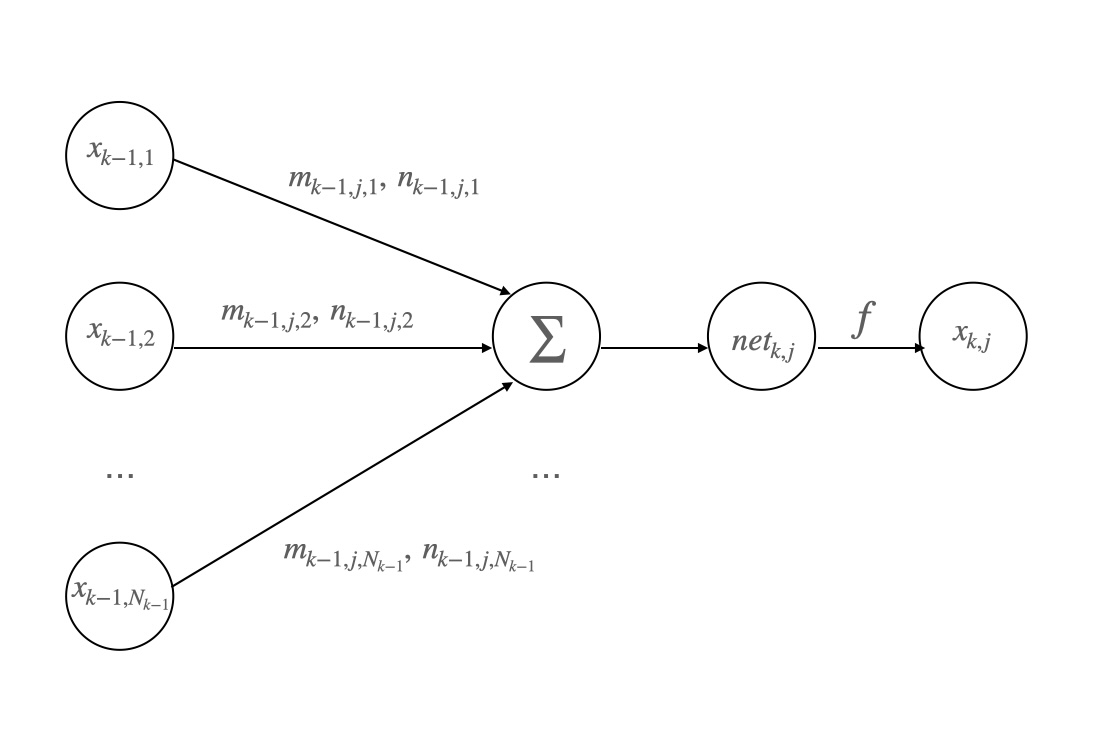
\includegraphics[width=0.8\linewidth]{hw4-figure1.jpg}
    \caption{第二题的神经网络}
\end{figure}

\begin{enumerate}
    \item 假定第$k$层的激活函数是sigmoid函数,那么第$k$层第$j$个神经元输出的信号$x_{k,j}$等于什么?(可以用$net_{k,j}$表示结果)。
    \item 假定我们计算该网络的输出后,得到其loss为$E$,我们第$k$层的第$j$个神经元从网络输出处反向传播而来的梯度为
\begin{equation}
    \frac{\partial E}{\partial x_{k, j}} = G_{k, j}
\end{equation}
    \item 请计算对于$net_{k, j}$的反向梯度$\frac{\partial E}{\partial net_{k, j}}$。要求用$G_{k,j}$与$x_{k,j}$表示该反向梯度。
    
    提示:sigmoid函数求导公式:$\frac{\partial sigmoid(x)}{\partial x} = sigmoid(x)\cdot [1-sigmoid(x)]$。
    \item 利用上方计算好的梯度$\frac{\partial E}{\partial net_{k, j}}$表达式计算参数$u_{k,j,i}$处的梯度$\frac{\partial E}{\partial m_{k,j,i}}$。要求用$G_{k,j}$与$x_{k,j}$表示该反向梯度。
    \item 假如该神经网络的学习率为$\eta$,那么参数$m_{k, j, i}$更新后的值$m'_{k, j, i}$为多少?要求用$G_{k,j}$,$x_{k,j}$, $m_{k, j, i}$与$\eta$表示更新后的参数。
\end{enumerate}

\begin{solution}
    
\end{solution}

\begin{problem}
    我们在lecture14中学习了层次化聚类(hierarchical clustering,HAC),k-means,dbscan密度聚类三种聚类方法,请比较一下这三种算法的时间复杂度和优缺点(假定计算两点之间的距离时间复杂度为$O(1)$)。
\end{problem}

\begin{solution}
    
\end{solution}

\end{document}